\documentclass[11pt]{article}

\usepackage[utf8]{inputenc}
\usepackage{graphicx}
\usepackage{hyperref}
\usepackage{enumitem}
\usepackage{scrextend}
\usepackage{titlesec}

\usepackage[top=0.7in,bottom=0.7in,left=0.75in,right=0.75in]{geometry}

\newcommand{\email}{joel.oskarsson@outlook.com}

\titleformat{\section}{\normalfont\large\bfseries}{\thesection}{1em}{}[\titlerule]
\titlespacing*{\section}{0pt}{7pt}{3pt}
\titleformat{\subsection}{\normalfont\normalsize\bfseries\itshape}{\thesubsection}{1em}{}
\titlespacing*{\subsection}{0pt}{5pt}{2pt}

\graphicspath{{./graphics/}}
\pagenumbering{gobble}

\setlength{\parindent}{0pt}
\setlist{noitemsep, topsep=0pt, parsep=0pt}

\begin{document}

% ===== Header =====
\noindent\begin{minipage}[c]{0.2\textwidth}
    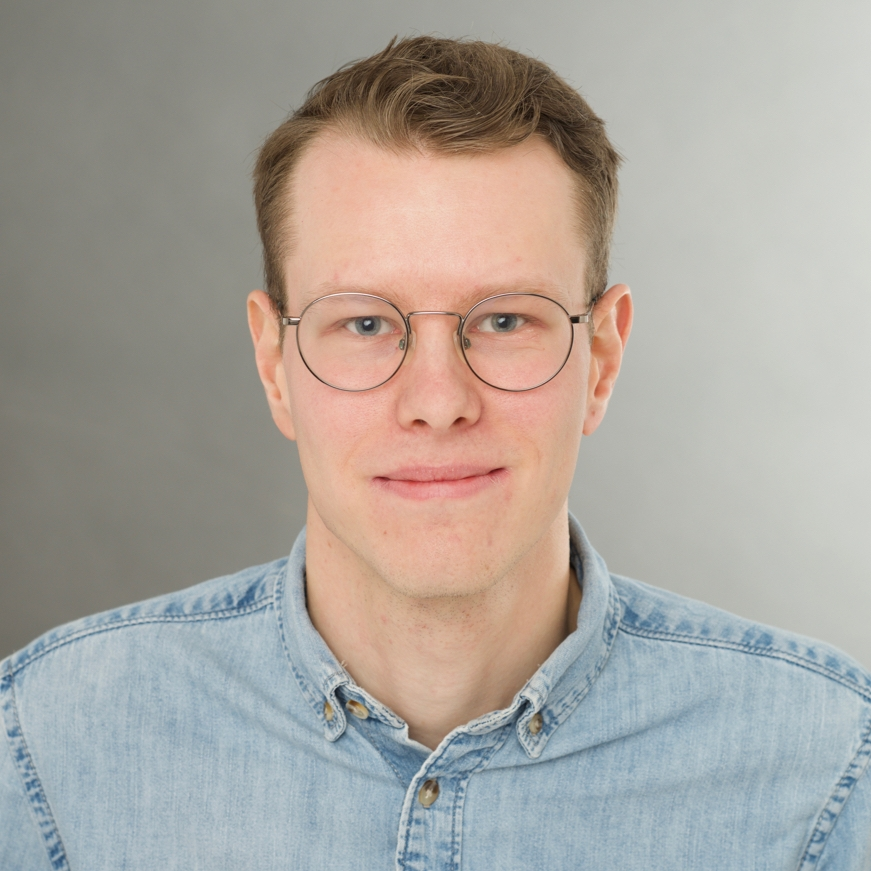
\includegraphics[height=3cm]{photo}
\end{minipage}%
\hspace{0.03\textwidth}%
\begin{minipage}[c]{0.77\textwidth}
    {\LARGE\textbf{Joel Oskarsson}}\\[4pt]
    \href{mailto:\email}{\email} $\cdot$ +41\,77\,289\,1572\\[2pt]
    \href{http://joeloskarsson.github.io}{joeloskarsson.github.io} $\cdot$ \href{http://linkedin.com/in/joel-oskarsson}{linkedin.com/in/joel-oskarsson}\\[2pt]
    ETH Zurich AI Center, Zurich, Switzerland\\[2pt]
    {\small Swedish (native) $\cdot$ English (fluent) $\cdot$ German (basic, A2)}
\end{minipage}

%\vspace{6pt}\hrule\vspace{4pt}

% ===== Employment and Education =====
\section*{Academic Career}
\begin{labeling}{2020--2025}
    \item [2025 --] \textbf{Postdoctoral Fellow, ETH Zurich AI Center}, Zurich, Switzerland
        \begin{itemize}
            \item Awarded 2-year fellowship in highly competitive call with a \textbf{4\% acceptance rate}.
            \item Mentored by Torsten Hoefler (Computer Science), Siddhartha Mishra (Math), and Benedikt Soja (Space Geodesy).
            Topic: \textit{Modeling the Earth System in Latent Space}.
            \item Funded by the Swiss AI Initiative, part of effort to develop \textbf{AI foundation models}.
        \end{itemize}
    \item [2020--2025] \textbf{PhD in Computer Science, Linköping University}, 240 ECTS
        \begin{itemize}
            \item Thesis: \href{https://urn.kb.se/resolve?urn=urn:nbn:se:liu:diva-215665}{\textit{Modeling Spatio-Temporal Systems with Graph-based Machine Learning}}
            \item Supervised by Fredrik Lindsten, Per Sidén, Tomas Landelius. 
            \item Affiliated with WASP graduate school.
        \end{itemize}
    \item [2015--2020] \textbf{Master's in Computer Science and Engineering, Linköping University}, 300 ECTS
        \begin{itemize}
            %\item Thesis: \href{http://urn.kb.se/resolve?urn=urn:nbn:se:liu:diva-166637}{\textit{Probabilistic Regression using Conditional Generative Adversarial Networks}}.
            \item \textbf{Exchange year at ETH Zurich}, Zurich, Switzerland (2018--2019).
            %\item Employed as teaching assistant for courses in computer science and mathematics, during multiple periods (2016--2019).
            %\item Completed summer internship at Ericsson Research, working on GNSS positioning (2018).
        \end{itemize}
\end{labeling}

\section*{Research}
\subsection*{Summary of publications}
{\footnotesize\textit{See separate document for full list of publications.}}

\begin{itemize}
    \item 6 conference papers, 2 journal papers, 7 workshop papers, 3 works under review.
    \item 425 total citations, h-index 9 (from Google Scholar, November 2026).
\end{itemize}

% ===== Grants =====
\subsection*{Awarded Research and Career Grants}
\begin{itemize}
    \item Co-applicant for ICAIN-IGAIP project grant (320{,}000 CHF $\approx$ 345{,}000 EUR, \textbf{4/40 applications funded}, 2026).\\
        {\footnotesize Project \textit{AI-Powered Early Warning and Profiling for Displaced Populations}, with Christina Humer (PI, ETHZ) and the International Organization for Migration.}
    \item Research visit scholarship ($60{,}000$ SEK $\approx 5{,}200$ EUR), WASP Program. %Wallenberg AI, Autonomous Systems and Software Program (WASP).
    \item Co-author of compute grants from NSC, Sweden and CSCS, Switzerland.
\end{itemize}

% ===== Invited Talks =====
\subsection*{Invited Talks}
\newcommand{\talk}[4]{%
    \item [#2] #3\\
    {\footnotesize\textit{#1}}
}
\newcommand{\shorttalk}[4]{%
    #3 (#2)%
}
%I have been invited to present my research at universities, research institutes and industry, including:
\begin{labeling}{2026}
\setlength{\itemsep}{1pt}
    \talk{GNNs for Spatio-Temporal and Earth System Modeling}{2026}{KCDS Summer School on Graph Neural Networks, Karlsruhe Institute of Technology (KIT)}{Karlsruhe, Germany}
    \talk{Probabilistic Weather Forecasting with Hierarchical Graph Neural Networks}{2025}{\textbf{Google DeepMind}}{Online}
    \talk{Frontiers in Machine Learning for Weather Forecasting}{2024}{RISE Learning Machines Seminars}{Online}
    \talk{Graph-based Machine Learning for Weather}{}{\textbf{European Centre for Medium-Range Weather Forecasts (ECMWF)}}{Bonn, Germany}
    \talk{Graph-based Machine Learning for Spatio-Temporal Data, with Application to Traffic and Weather Forecasting}{}{\textbf{University of New South Wales (UNSW)}}{Sydney, Australia (Online)}
\end{labeling}
{\footnotesize
Selected further invited talks:
\shorttalk{Probabilistic Deep Learning for Earth System Modeling}{2026}{WeatherGenerator Dissemination Workshop}{Oslo, Norway};
\shorttalk{Graph-based Neural Weather Prediction for Limited Area Modeling}{2024}{MeteoSwiss}{Zurich, Switzerland};
\shorttalk{Graph-based Neural Weather Prediction for Limited Area Modeling}{2024}{ETH Zurich}{Zurich, Switzerland};
\shorttalk{Graph-based Neural Weather Prediction for Limited Area Modeling}{2024}{Uppsala University}{Uppsala, Sweden};
\shorttalk{Graph-based Neural Weather Prediction for Limited Area Modeling}{2023}{Danish Meteorological Institute}{Copenhagen, Denmark}.
}

% ===== Software =====
\subsection*{Software Research Output}
Creator and maintainer of the \href{https://github.com/mllam/neural-lam}{\textit{Neural-LAM}} \textbf{open source library} for AI weather forecasting research.
\begin{itemize}
    \item Translates research findings into direct community impact through open-source tooling.
    \item \textbf{Over 300 GitHub forks and stars}, reflecting widespread usage.
    \item Used by multiple \textbf{international research groups}, basis for many peer-reviewed publications.
    \item Organizational participant in Google Summer of Code 2026, personally acting as project mentor.
\end{itemize}

% ===== Research Visits =====
\subsection*{Research Visits}
\begin{labeling}{2023\quad}
\item [2023] Five-week research visit to \textbf{University College London (UCL)}, London, U.K.\\
        {\footnotesize Hosted by Prof.\ Marc Deisenroth, Sustainability and Machine Learning Group.}
\end{labeling}
\vspace{-1em}
{\footnotesize
Shorter visits:
Norwegian Meteorological Institute, Oslo (2026);
ECMWF, Bonn (2024);
ETH Zurich + MeteoSwiss, Zurich (2024);
Finnish Center for AI + Aalto University, Helsinki (2022, WASP International Study Visit).
}

% ===== Scientific Events =====
\subsection*{Presentations at Scientific Events (Highlights)}
\begin{itemize}
    \item Presentations at top \textbf{machine learning conferences}, and accompanying workshops:
        NeurIPS (2024: poster; 2023: workshop poster),
        ICML (2024: workshop poster),
        AISTATS (2023: poster).
    \item Selected for \textbf{oral presentations} at the Machine Learning for Earth System Modelling Workshop, Bonn, Germany, in \textbf{three consecutive years} (2023, 2024, 2025).
    \item Oral presentations at the Climate Informatics Conference, Lausanne, Switzerland (2026) and the KVA Symposium on AI for Science, Stockholm (2025)
    %\item Oral presentation, poster and panel discussion at the ESA-ECMWF Workshop on Machine Learning for Earth Observation, Frascati, Italy (2024)
\end{itemize}
\iffalse
    {\footnotesize
    Selected further presentations:
    Climate Informatics, Lausanne, Switzerland (2026, oral);
    Learning on Graphs and Geometry Meetup, Uppsala (2025, oral);
    %ELLIIT Focus Period: ML for Climate Science, Linköping (2024, poster);
    NORDSTAT, Gothenburg (2023, oral);
    Swedish Symposium on Image Analysis and Deep Learning, Norrköping (2023, poster);
    %Nordic Probabilistic AI Summer School, Helsinki, Finland (2022, poster).
    }
\fi

% ===== Other Academic Activities =====
\section*{Community and Academic Service}
% ===== Reviewing =====
\subsection*{Reviewing and Editorial Service}
{\footnotesize
\textbf{Area chair:} ICLR (2027).\\
\textbf{Reviewer:} NeurIPS (2024; 2026 -- \textit{Top Reviewer}); ICLR (2025, 2026); AISTATS (2023, 2024, 2026); Climate Informatics (2026); Geoscientific Model Development (2026); Quarterly Journal of the Royal Meteorological Society (2026); Geophysical Research Letters (2025); SOLA (2025); Geomatics, Natural Hazards and Risk (2025, 2026); CCAI workshop (2024, 2025).
}

\subsection*{Organizing and Other Service}
{\footnotesize
\begin{labeling}{2023--2025}
    \item [2026] Co-organizer of the \href{https://ai-environment-summit.com/}{\textit{AI + Environment Summit 2026}}, Zurich. Responsible for session on AI for weather and climate, and poster session.
    \item [2025--2026] Reviewer for applications to ETH Zurich AI Center Fellowship 2026.
    \item [2023--2025] Co-organizer of monthly online meetups for ML limited area weather forecasting researchers.
    \item [2022--2025] Organizer of the \href{https://github.com/STIMALiU/ml-reading-group}{\textit{STIMA ML Reading Group}}, Linköping University.
\end{labeling}
}

% ===== Teaching and Supervision =====
\section*{Teaching, Supervision and Mentoring}
%I enjoy teaching the fundamentals of machine learning and mentoring students to work on topics close to my research interests.
\begin{itemize}
    \item Supervisor of \textbf{10 master's theses} (8 LiU and 2 ETHZ, 1 ongoing) and 1 bachelor's thesis (ETHZ, ongoing).
    \item Mentored junior PhD students through collaborative research, co-authorship, and project guidance.
    \item Co- and guest-lecturer for courses \textit{AI Center Projects in Machine Learning Research} (ETHZ) and \textit{Time Series and Sequence Learning} (LiU).
    \item \textbf{Co-course-developer} of the \href{https://foundations-of-ml.ida.liu.se/}{\textit{Foundations of Machine Learning}} online course (LiU, 2021--2024).
    \item Pedagogical training: \textit{Becoming a Teacher in Higher Education}, 6 ECTS (LiU, 2021).
\end{itemize}
{\footnotesize
Other teaching assistant work (2016--2024): Advanced Machine Learning ($5\times$), Computational Statistics, Foundations of ML, Building AI, Introduction to Python, etc. All at LiU.
}
% ===== Media Coverage and Scientific Outreach =====
\section*{Media Coverage and Scientific Outreach}
\begin{itemize}
    \item \textit{AI för prognosmeteorologer} (2025): Lecture for forecast meteorologists about AI weather forecasting.
    \item \textit{Forskningsframsteg inom Maskininlärning för Väderprognoser} (2025): \textbf{Popular science article} in Polarfront, journal of the Swedish meteorological society.
    \item \href{https://www.svt.se/nyheter/lokalt/ost/de-vill-gora-vaderprognoser-mer-palitliga-med-hjalp-av-ai}{\textit{De vill göra väderprognoser mer pålitliga -- med hjälp av AI}}, SVT (2024): \textbf{Television news feature}.
    \item \href{https://liu.se/artikel/forbattrade-vaderprognoser-med-ai}{\textit{Förbättrade väderprognoser med AI}}, Linköping University (2023): News article on University website.
    %\item \textit{Doing a PhD in Machine Learning and AI within WASP} (2025): Talk for undergraduate students.
\end{itemize}

\end{document}
